\documentclass[12pt,a4paper,titlepage]{article}
\usepackage{lab_style}
\usepackage{pdfpages}
\usepackage{eso-pic}
\usepackage{graphicx}
\usepackage{float}
\newcommand\tab[1][1cm]{\hspace*{#1}}

\graphicspath{ {./} }
  
\begin{document}

\begin{titlepage}
\selectlanguage{english}

%----------------------------------------------------------------------------------------
% TITLE PAGE INFORMATION
%----------------------------------------------------------------------------------------
  \begin{center} % Center everything on the page

  %----------------------------------------------------------------------------------------
  % HEADING SECTIONS
  %----------------------------------------------------------------------------------------
  \textsc{\large Faculty of Computers, Informatics and Microelectronics}\\[0.5cm]
  \textsc{\large Technical University of Moldova}\\[1.2cm] % Name of your university/college
  \vspace{25 mm}

  \textsc{\Large Object-Oriented Modeling and Analysis}\\[0.5cm] % Major heading such as course name
  \textsc{\large Laboratory work \#6}\\[0.5cm] % Minor heading such as course title

\newcommand{\HRule}{\rule{\linewidth}{0.5mm}} % Defines a new command for the horizontal lines, change thickness here

  %----------------------------------------------------------------------------------------
  % TITLE SECTION
  %----------------------------------------------------------------------------------------
  \vspace{10 mm}
  \HRule \\[0.4cm]
  { \LARGE \bfseries Modeling your project with Statechart Diagrams. Domain Analysis. SOLID / GRASP Prin-
ciples. }\\[0.4cm] % Title of your document
  \HRule \\[1.5cm]

  %----------------------------------------------------------------------------------------
  % AUTHOR SECTION
  %----------------------------------------------------------------------------------------
      \vspace{30mm}

      \begin{minipage}{0.4\textwidth}
      \begin{flushleft} \large
      \emph{Author:}\\
      Cernei \textsc{Liviu}
      \end{flushleft}
      \end{minipage}
      ~
      \begin{minipage}{0.4\textwidth}
      \begin{flushright} \large
      \emph{Supervisor:} \\
      Mihail \textsc{Gavrilița} % Supervisor's Name
      \end{flushright}
      \end{minipage}\\[4cm]

      \vspace{5 mm}
      % If you don't want a supervisor, uncomment the two lines below and remove the section above
      %\Large \emph{Author:}\\
      %John \textsc{Smith}\\[3cm] % Your name

      %----------------------------------------------------------------------------------------
      % DATE SECTION
      %----------------------------------------------------------------------------------------

      {\large Chișinau 2018}\\[3cm] % Date, change the \today to a set date if you want to be precise

      %----------------------------------------------------------------------------------------
      % LOGO SECTION
      %----------------------------------------------------------------------------------------

      %\includegraphics{red}\\[0.5cm] % Include a department/university logo - this will require the graphicx package

      %----------------------------------------------------------------------------------------

      \vfill % Fill the rest of the page with whitespace
      \end{center}
      
\end{titlepage}

\cleardoublepage

\newpage

\pagenumbering{arabic}
\setcounter{page}{1}
\setcounter{secnumdepth}{4}

\addtocontents{toc}{\protect\thispagestyle{empty}} % no page number on the table of contents page
\cleardoublepage


\phantomsection
\addcontentsline{toc}{section}{Introduction}
\section*{Laboratory work \#6}
\phantomsection

\section{Tasks}
\begin{itemize}
	\item
	Model your application using 3 Statechart Diagrams;
	\item 
	Perform the Domain analysis of your project.
\end{itemize}

\section{Theory}

\subsection{SOLID / GRASP Principles.}
\textbf{SOLID Principles are principles of class design.}
\begin{itemize}
	\item SRP: Single Responsibility Principle–An object should have only a single responsibility and all the responsibility should be entirely encapsulated by the class.–There should never be more than one reason for a class to change
	\item OCP: Open/Closed Principle–Software entities should be open for extension, but closed for modification
	\item LSP: Liskov Substituion Principle–Objects in a program should be replaceable with instances of their subtypes without altering the correctness of that program
	\item ISP: Interface Segregation Principle–many client specific interfaces are better than one general purpose interface–once an interface has gotten too 'fat' split it into smaller and more specific interfaces so that any clients of the interface will only know about the methods that pertain to them. No client should be forced to depend on methods it does not use
	\item DIP: Dependency Inversion Principle–Depend upon Abstractions. Do not depend upon concretions.Dependency Injection (DI) is one method of following this principle.
\end{itemize}

\textbf{GRASP - Acronym for General Responsibility Assignment Software Patterns.}
\begin{itemize}
	\item Assigning responsibilities to classes is a critical aspect of object-oriented design.
	\item Appropriate assignment of responsibilities to classes is the key to successful design.
	\item There are fundamental principles in assigning responsibilities that experienced designers apply.
	\item These principles are summarized in the GRASP patterns.
	\item Has nine core principles that object-oriented designers apply when assigning responsibilities to classes and designing message interactions.
\end{itemize}
\clearpage

\section{Statechart Diagrams}
In Figure ~\ref{fig:userAccount} is represented the statechart diagram for the user account.
\begin{figure}[H]
\centering
	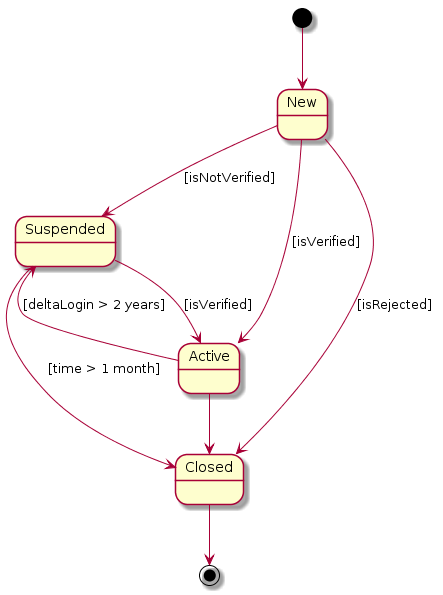
\includegraphics[width=10cm]{userAccount}
	\caption{User account statechart diagram}
	\label{fig:userAccount}
\end{figure}
Initially all accounts are new (initialization). Those who had valid usernames and passwords, receive a notification by mail. Other ones are rejected, then closed. If the user does not verify the account, it becomes suspended. Suspenden accounts can become active if are verified in less than a month, else they are also closed. An active account with an "Offline" status more than 2 years, becomes supended and receives a new mail notification. Closed accounts have the final state.

In Figure ~\ref{fig:courses} is represented the statechart diagram for courses.
\begin{figure}[H]
\centering
	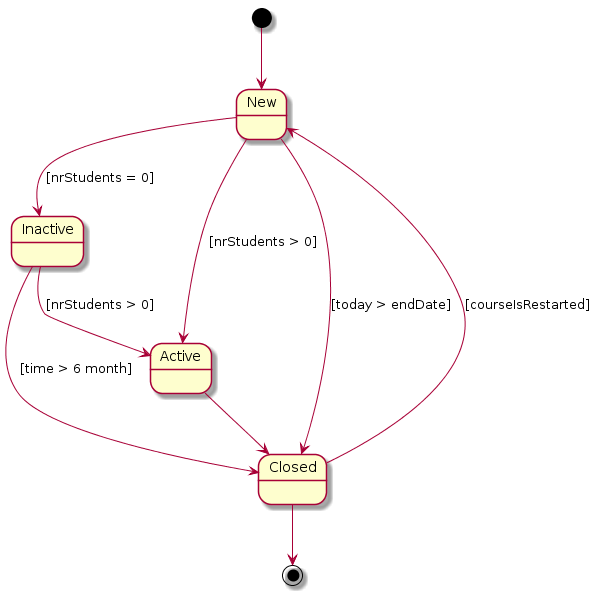
\includegraphics[width=10cm]{courses}
	\caption{Courses statechart diagram}
	\label{fig:courses}
\end{figure}
The teacher can create new courses. If he registers some users, the course becomes active. If there are no students at the beginning, the course is inactive. If he can't attract any students in half a year, the course is closed. If the starting date was incorect, the course is also closed. But any course can be restarted, if it was marked as closed.

In Figure ~\ref{fig:search} is represented the statechart diagram for searching a course.
\begin{figure}[H]
\centering
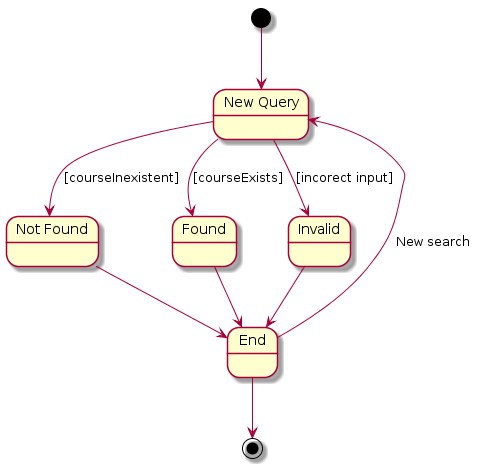
\includegraphics[width=10cm]{search}
\caption{Search operation statechart diagram}
\label{fig:search}
\end{figure}
An user who wants to search a course, creates a new query. If he inputs non-alfanumeric symbols, the result is invalidated. If the course is not found, the result is negative and a propper message appears. Otherwise, the course is found and a positive result with a success message is sent. All states then become finished.

\section{Domain analysis}
Online courses are aimed at unlimited participation and open access via the web. In addition to traditional course materials such as filmed lectures, readings, and problem sets, many online courses provide interactive user forums to support community interactions among students, professors, and teaching assistants (TAs).\par
Online courses are regarded by many as an important tool to widen access to Higher Education (HE) for millions of people, including those in the developing world, and ultimately enhance their quality of life. Online courses may be regarded as contributing to the democratisation of HE, not only locally or regionally but globally as well. Online courses can help democratise content and make knowledge reachable for everyone. Students are able to access complete courses offered by universities all over the world, something previously unattainable. With the availability of affordable technologies, online courses increase access to an extraordinary number of courses offered by world-renowned institutions and teachers.\par
There are already similar platforms. "Coursera" emerged as the top ranked online courses platform and the best overall choice due to its impressive selection of learning pathways and course features. "edX" and "Udacity" were also found to be strong contenders.
\section{Conclusion}
In this laboratory work we learned to create statechart diagrams and perform domain analysis.

\clearpage
\cleardoublepage

\end{document}
